\documentclass[1p]{elsarticle_modified}
%\bibliographystyle{elsarticle-num}

%\usepackage[colorlinks]{hyperref}
%\usepackage{abbrmath_seonhwa} %\Abb, \Ascr, \Acal ,\Abf, \Afrak
\usepackage{amsfonts}
\usepackage{amssymb}
\usepackage{amsmath}
\usepackage{amsthm}
\usepackage{scalefnt}
\usepackage{amsbsy}
\usepackage{kotex}
\usepackage{caption}
\usepackage{subfig}
\usepackage{color}
\usepackage{graphicx}
\usepackage{xcolor} %% white, black, red, green, blue, cyan, magenta, yellow
\usepackage{float}
\usepackage{setspace}
\usepackage{hyperref}

\usepackage{tikz}
\usetikzlibrary{arrows}

\usepackage{multirow}
\usepackage{array} % fixed length table
\usepackage{hhline}

%%%%%%%%%%%%%%%%%%%%%
\makeatletter
\renewcommand*\env@matrix[1][\arraystretch]{%
	\edef\arraystretch{#1}%
	\hskip -\arraycolsep
	\let\@ifnextchar\new@ifnextchar
	\array{*\c@MaxMatrixCols c}}
\makeatother %https://tex.stackexchange.com/questions/14071/how-can-i-increase-the-line-spacing-in-a-matrix
%%%%%%%%%%%%%%%

\usepackage[normalem]{ulem}

\newcommand{\msout}[1]{\ifmmode\text{\sout{\ensuremath{#1}}}\else\sout{#1}\fi}
%SOURCE: \msout is \stkout macro in https://tex.stackexchange.com/questions/20609/strikeout-in-math-mode

\newcommand{\cancel}[1]{
	\ifmmode
	{\color{red}\msout{#1}}
	\else
	{\color{red}\sout{#1}}
	\fi
}

\newcommand{\add}[1]{
	{\color{blue}\uwave{#1}}
}

\newcommand{\replace}[2]{
	\ifmmode
	{\color{red}\msout{#1}}{\color{blue}\uwave{#2}}
	\else
	{\color{red}\sout{#1}}{\color{blue}\uwave{#2}}
	\fi
}

\newcommand{\Sol}{\mathcal{S}} %segment
\newcommand{\D}{D} %diagram
\newcommand{\A}{\mathcal{A}} %arc


%%%%%%%%%%%%%%%%%%%%%%%%%%%%%5 test

\def\sl{\operatorname{\textup{SL}}(2,\Cbb)}
\def\psl{\operatorname{\textup{PSL}}(2,\Cbb)}
\def\quan{\mkern 1mu \triangleright \mkern 1mu}

\theoremstyle{definition}
\newtheorem{thm}{Theorem}[section]
\newtheorem{prop}[thm]{Proposition}
\newtheorem{lem}[thm]{Lemma}
\newtheorem{ques}[thm]{Question}
\newtheorem{cor}[thm]{Corollary}
\newtheorem{defn}[thm]{Definition}
\newtheorem{exam}[thm]{Example}
\newtheorem{rmk}[thm]{Remark}
\newtheorem{alg}[thm]{Algorithm}

\newcommand{\I}{\sqrt{-1}}
\begin{document}

%\begin{frontmatter}
%
%\title{Boundary parabolic representations of knots up to 8 crossings}
%
%%% Group authors per affiliation:
%\author{Yunhi Cho} 
%\address{Department of Mathematics, University of Seoul, Seoul, Korea}
%\ead{yhcho@uos.ac.kr}
%
%
%\author{Seonhwa Kim} %\fnref{s_kim}}
%\address{Center for Geometry and Physics, Institute for Basic Science, Pohang, 37673, Korea}
%\ead{ryeona17@ibs.re.kr}
%
%\author{Hyuk Kim}
%\address{Department of Mathematical Sciences, Seoul National University, Seoul 08826, Korea}
%\ead{hyukkim@snu.ac.kr}
%
%\author{Seokbeom Yoon}
%\address{Department of Mathematical Sciences, Seoul National University, Seoul, 08826,  Korea}
%\ead{sbyoon15@snu.ac.kr}
%
%\begin{abstract}
%We find all boundary parabolic representation of knots up to 8 crossings.
%
%\end{abstract}
%\begin{keyword}
%    \MSC[2010] 57M25 
%\end{keyword}
%
%\end{frontmatter}

%\linenumbers
%\tableofcontents
%
\newcommand\colored[1]{\textcolor{white}{\rule[-0.35ex]{0.8em}{1.4ex}}\kern-0.8em\color{red} #1}%
%\newcommand\colored[1]{\textcolor{white}{ #1}\kern-2.17ex	\textcolor{white}{ #1}\kern-1.81ex	\textcolor{white}{ #1}\kern-2.15ex\color{red}#1	}

{\Large $\underline{11a_{249}~(K11a_{249})}$}

\setlength{\tabcolsep}{10pt}
\renewcommand{\arraystretch}{1.6}
\vspace{1cm}\begin{tabular}{m{100pt}>{\centering\arraybackslash}m{274pt}}
\multirow{5}{120pt}{
	\centering
	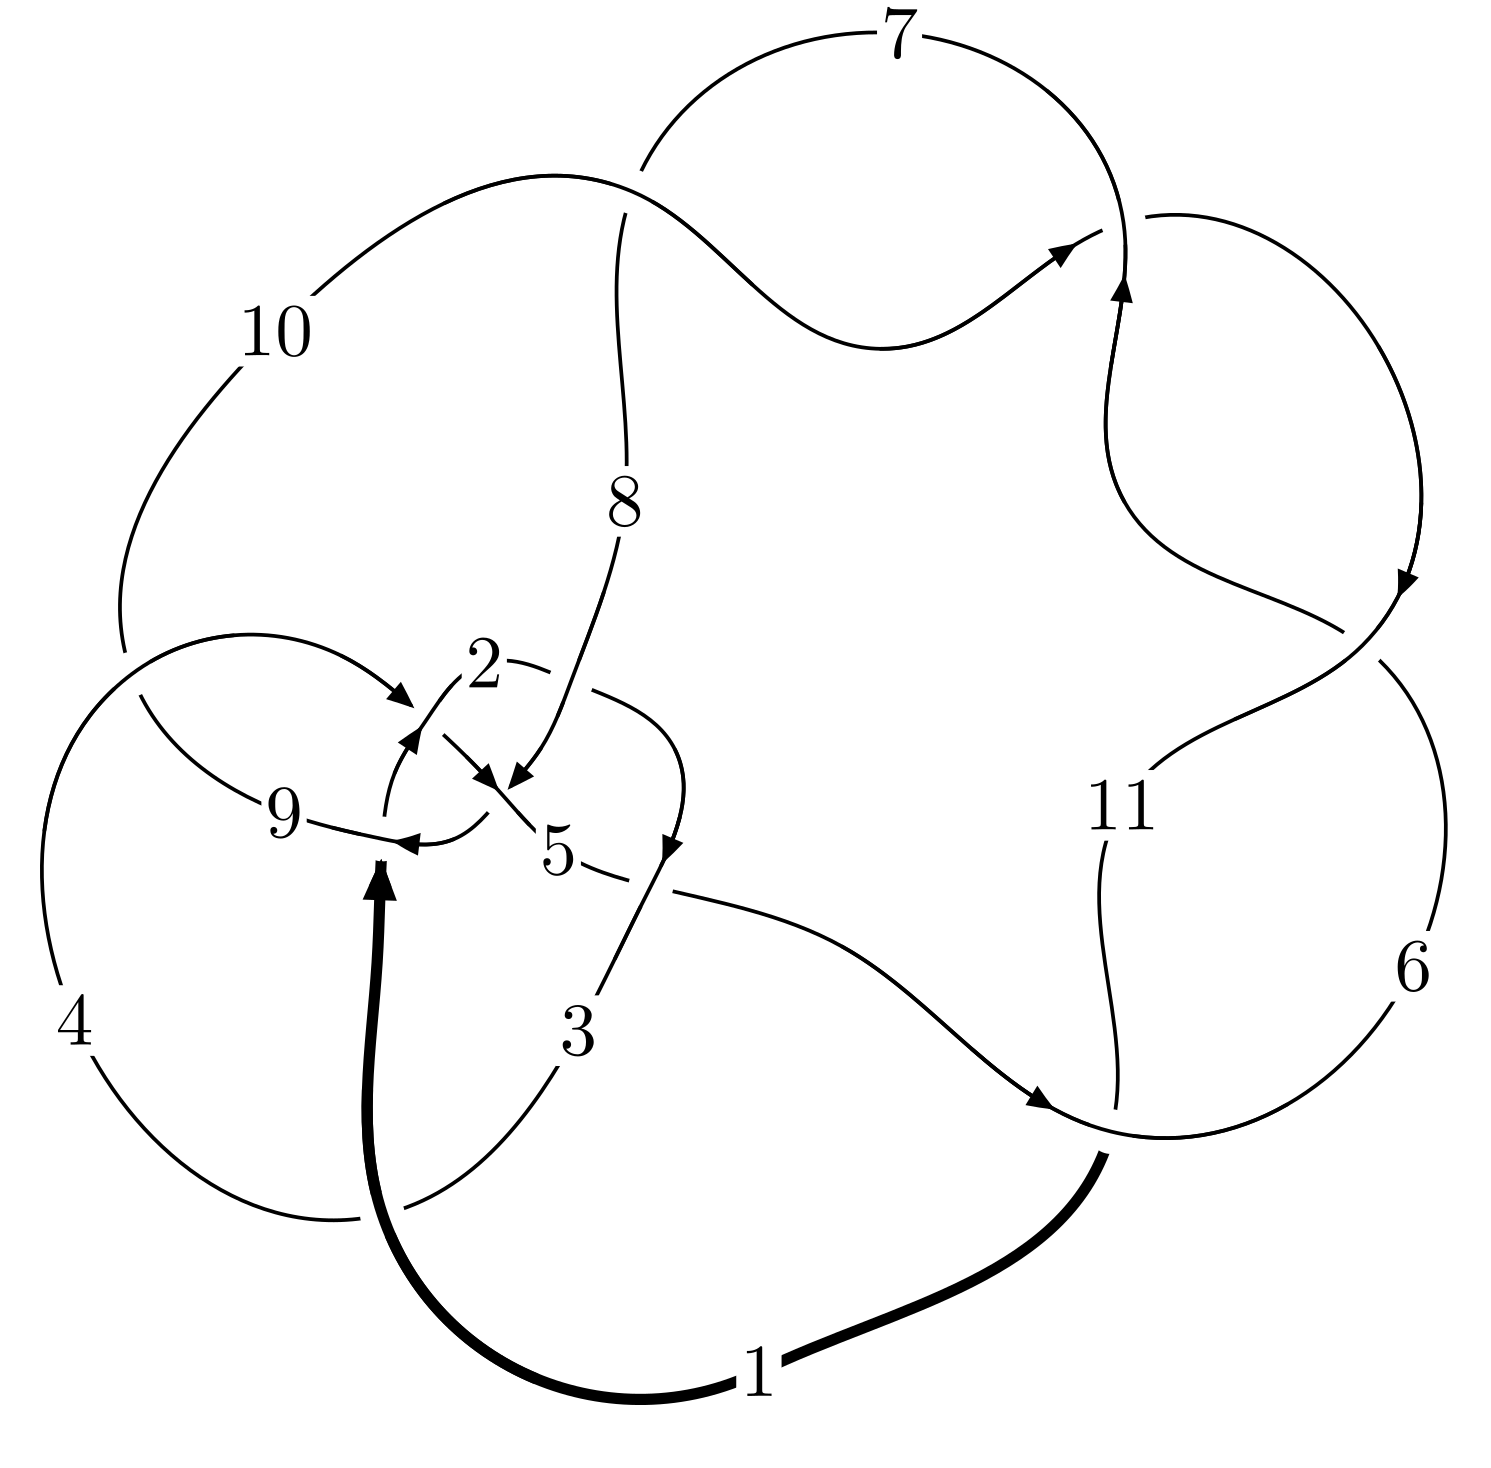
\includegraphics[width=112pt]{../../../GIT/diagram.site/Diagrams/png/498_11a_249.png}\\
\ \ \ A knot diagram\footnotemark}&
\allowdisplaybreaks
\textbf{Linearized knot diagam} \\
\cline{2-2}
 &
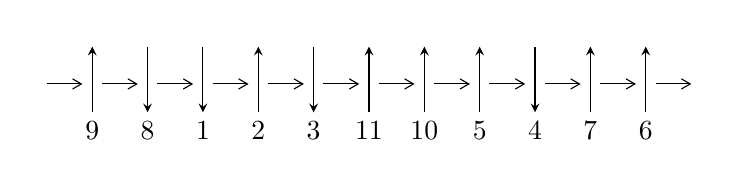
\begin{tikzpicture}[x=20pt, y=17pt]
	% nodes
	\node (C0) at (0, 0) {};
	\node (C1) at (1, 0) {};
	\node (C1U) at (1, +1) {};
	\node (C1D) at (1, -1) {9};

	\node (C2) at (2, 0) {};
	\node (C2U) at (2, +1) {};
	\node (C2D) at (2, -1) {8};

	\node (C3) at (3, 0) {};
	\node (C3U) at (3, +1) {};
	\node (C3D) at (3, -1) {1};

	\node (C4) at (4, 0) {};
	\node (C4U) at (4, +1) {};
	\node (C4D) at (4, -1) {2};

	\node (C5) at (5, 0) {};
	\node (C5U) at (5, +1) {};
	\node (C5D) at (5, -1) {3};

	\node (C6) at (6, 0) {};
	\node (C6U) at (6, +1) {};
	\node (C6D) at (6, -1) {11};

	\node (C7) at (7, 0) {};
	\node (C7U) at (7, +1) {};
	\node (C7D) at (7, -1) {10};

	\node (C8) at (8, 0) {};
	\node (C8U) at (8, +1) {};
	\node (C8D) at (8, -1) {5};

	\node (C9) at (9, 0) {};
	\node (C9U) at (9, +1) {};
	\node (C9D) at (9, -1) {4};

	\node (C10) at (10, 0) {};
	\node (C10U) at (10, +1) {};
	\node (C10D) at (10, -1) {7};

	\node (C11) at (11, 0) {};
	\node (C11U) at (11, +1) {};
	\node (C11D) at (11, -1) {6};
	\node (C12) at (12, 0) {};

	% arrows
	\draw[->,>={angle 60}]
	(C0) edge (C1) (C1) edge (C2) (C2) edge (C3) (C3) edge (C4) (C4) edge (C5) (C5) edge (C6) (C6) edge (C7) (C7) edge (C8) (C8) edge (C9) (C9) edge (C10) (C10) edge (C11) (C11) edge (C12) ;	\draw[->,>=stealth]
	(C1D) edge (C1U) (C2U) edge (C2D) (C3U) edge (C3D) (C4D) edge (C4U) (C5U) edge (C5D) (C6D) edge (C6U) (C7D) edge (C7U) (C8D) edge (C8U) (C9U) edge (C9D) (C10D) edge (C10U) (C11D) edge (C11U) ;
	\end{tikzpicture} \\
\hhline{~~} \\& 
\textbf{Solving Sequence} \\ \cline{2-2} 
 &
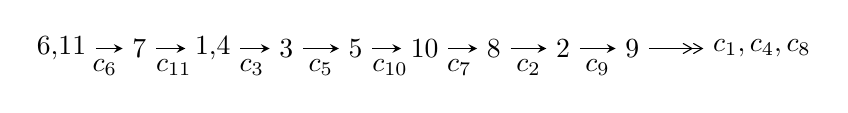
\begin{tikzpicture}[x=25pt, y=7pt]
	% node
	\node (A0) at (-1/8, 0) {6,11};
	\node (A1) at (1, 0) {7};
	\node (A2) at (33/16, 0) {1,4};
	\node (A3) at (25/8, 0) {3};
	\node (A4) at (33/8, 0) {5};
	\node (A5) at (41/8, 0) {10};
	\node (A6) at (49/8, 0) {8};
	\node (A7) at (57/8, 0) {2};
	\node (A8) at (65/8, 0) {9};
	\node (C1) at (1/2, -1) {$c_{6}$};
	\node (C2) at (3/2, -1) {$c_{11}$};
	\node (C3) at (21/8, -1) {$c_{3}$};
	\node (C4) at (29/8, -1) {$c_{5}$};
	\node (C5) at (37/8, -1) {$c_{10}$};
	\node (C6) at (45/8, -1) {$c_{7}$};
	\node (C7) at (53/8, -1) {$c_{2}$};
	\node (C8) at (61/8, -1) {$c_{9}$};
	\node (A9) at (10, 0) {$c_{1},c_{4},c_{8}$};

	% edge
	\draw[->,>=stealth]	
	(A0) edge (A1) (A1) edge (A2) (A2) edge (A3) (A3) edge (A4) (A4) edge (A5) (A5) edge (A6) (A6) edge (A7) (A7) edge (A8) ;
	\draw[->>,>={angle 60}]	
	(A8) edge (A9);
\end{tikzpicture} \\ 

\end{tabular} \\

\footnotetext{
The image of knot diagram is generated by the software ``\textbf{Draw programme}" developed by Andrew Bartholomew(\url{http://www.layer8.co.uk/maths/draw/index.htm\#Running-draw}), where we modified some parts for our purpose(\url{https://github.com/CATsTAILs/LinksPainter}).
}\phantom \\ \newline 
\centering \textbf{Ideals for irreducible components\footnotemark of $X_{\text{par}}$} 
 
\begin{align*}
I^u_{1}&=\langle 
-2221 u^{30}+10362 u^{29}+\cdots+1483 b+12391,\;16251 u^{30}-71483 u^{29}+\cdots+5932 a-87087,\\
\phantom{I^u_{1}}&\phantom{= \langle  }u^{31}-5 u^{30}+\cdots-29 u+4\rangle \\
I^u_{2}&=\langle 
- u^{17} a+u^{18}+\cdots+b- a,\;- u^{18}-2 u^{17}+\cdots+a+3,\;u^{19}+3 u^{18}+\cdots+2 u+1\rangle \\
I^u_{3}&=\langle 
- u^8-3 u^7-8 u^6-14 u^5-18 u^4-18 u^3-12 u^2+b-5 u-1,\\
\phantom{I^u_{3}}&\phantom{= \langle  }u^{10}+2 u^9+8 u^8+11 u^7+20 u^6+18 u^5+16 u^4+7 u^3- u^2+a-2 u-3,\\
\phantom{I^u_{3}}&\phantom{= \langle  }u^{11}+2 u^{10}+9 u^9+14 u^8+29 u^7+34 u^6+40 u^5+33 u^4+21 u^3+11 u^2+2 u+1\rangle \\
\\
\end{align*}
\raggedright * 3 irreducible components of $\dim_{\mathbb{C}}=0$, with total 80 representations.\\
\footnotetext{All coefficients of polynomials are rational numbers. But the coefficients are sometimes approximated in decimal forms when there is not enough margin.}
\newpage
\renewcommand{\arraystretch}{1}
\centering \section*{I. $I^u_{1}= \langle -2221 u^{30}+10362 u^{29}+\cdots+1483 b+12391,\;16251 u^{30}-71483 u^{29}+\cdots+5932 a-87087,\;u^{31}-5 u^{30}+\cdots-29 u+4 \rangle$}
\flushleft \textbf{(i) Arc colorings}\\
\begin{tabular}{m{7pt} m{180pt} m{7pt} m{180pt} }
\flushright $a_{6}=$&$\begin{pmatrix}1\\0\end{pmatrix}$ \\
\flushright $a_{11}=$&$\begin{pmatrix}0\\u\end{pmatrix}$ \\
\flushright $a_{7}=$&$\begin{pmatrix}1\\- u^2\end{pmatrix}$ \\
\flushright $a_{1}=$&$\begin{pmatrix}u\\u\end{pmatrix}$ \\
\flushright $a_{4}=$&$\begin{pmatrix}-2.73955 u^{30}+12.0504 u^{29}+\cdots-82.3793 u+14.6809\\1.49764 u^{30}-6.98719 u^{29}+\cdots+54.4889 u-8.35536\end{pmatrix}$ \\
\flushright $a_{3}=$&$\begin{pmatrix}-2.08884 u^{30}+8.94656 u^{29}+\cdots-37.0260 u+6.08749\\2.14835 u^{30}-10.0910 u^{29}+\cdots+99.8422 u-16.9488\end{pmatrix}$ \\
\flushright $a_{5}=$&$\begin{pmatrix}3.62053 u^{30}-14.7615 u^{29}+\cdots+60.7468 u-11.9584\\-4.83884 u^{30}+22.6966 u^{29}+\cdots-198.526 u+33.8375\end{pmatrix}$ \\
\flushright $a_{10}=$&$\begin{pmatrix}- u\\u^3+u\end{pmatrix}$ \\
\flushright $a_{8}=$&$\begin{pmatrix}u^2+1\\- u^4-2 u^2\end{pmatrix}$ \\
\flushright $a_{2}=$&$\begin{pmatrix}-0.160991 u^{30}+0.195381 u^{29}+\cdots+25.2053 u-4.91925\\1.19285 u^{30}-5.61834 u^{29}+\cdots+51.1949 u-8.53338\end{pmatrix}$ \\
\flushright $a_{9}=$&$\begin{pmatrix}2.95499 u^{30}-13.1485 u^{29}+\cdots+127.609 u-25.1701\\-0.175320 u^{30}+1.38031 u^{29}+\cdots-36.5408 u+8.03034\end{pmatrix}$\\ \flushright $a_{9}=$&$\begin{pmatrix}2.95499 u^{30}-13.1485 u^{29}+\cdots+127.609 u-25.1701\\-0.175320 u^{30}+1.38031 u^{29}+\cdots-36.5408 u+8.03034\end{pmatrix}$\\&\end{tabular}
\flushleft \textbf{(ii) Obstruction class $= -1$}\\~\\
\flushleft \textbf{(iii) Cusp Shapes $= \frac{23165}{1483} u^{30}-\frac{107745}{1483} u^{29}+\cdots+\frac{898798}{1483} u-\frac{164430}{1483}$}\\~\\
\newpage\renewcommand{\arraystretch}{1}
\flushleft \textbf{(iv) u-Polynomials at the component}\newline \\
\begin{tabular}{m{50pt}|m{274pt}}
Crossings & \hspace{64pt}u-Polynomials at each crossing \\
\hline $$\begin{aligned}c_{1},c_{8}\end{aligned}$$&$\begin{aligned}
&u^{31}- u^{30}+\cdots+u-1
\end{aligned}$\\
\hline $$\begin{aligned}c_{2},c_{9}\end{aligned}$$&$\begin{aligned}
&u^{31}- u^{29}+\cdots- u-2
\end{aligned}$\\
\hline $$\begin{aligned}c_{3},c_{5}\end{aligned}$$&$\begin{aligned}
&u^{31}+4 u^{30}+\cdots+18 u-1
\end{aligned}$\\
\hline $$\begin{aligned}c_{4}\end{aligned}$$&$\begin{aligned}
&u^{31}+18 u^{30}+\cdots+9 u+2
\end{aligned}$\\
\hline $$\begin{aligned}c_{6},c_{7},c_{10}\\c_{11}\end{aligned}$$&$\begin{aligned}
&u^{31}+5 u^{30}+\cdots-29 u-4
\end{aligned}$\\
\hline
\end{tabular}\\~\\
\newpage\renewcommand{\arraystretch}{1}
\flushleft \textbf{(v) Riley Polynomials at the component}\newline \\
\begin{tabular}{m{50pt}|m{274pt}}
Crossings & \hspace{64pt}Riley Polynomials at each crossing \\
\hline $$\begin{aligned}c_{1},c_{8}\end{aligned}$$&$\begin{aligned}
&y^{31}+13 y^{30}+\cdots-33 y-1
\end{aligned}$\\
\hline $$\begin{aligned}c_{2},c_{9}\end{aligned}$$&$\begin{aligned}
&y^{31}-2 y^{30}+\cdots+77 y-4
\end{aligned}$\\
\hline $$\begin{aligned}c_{3},c_{5}\end{aligned}$$&$\begin{aligned}
&y^{31}-26 y^{30}+\cdots+92 y-1
\end{aligned}$\\
\hline $$\begin{aligned}c_{4}\end{aligned}$$&$\begin{aligned}
&y^{31}+36 y^{29}+\cdots-43 y-4
\end{aligned}$\\
\hline $$\begin{aligned}c_{6},c_{7},c_{10}\\c_{11}\end{aligned}$$&$\begin{aligned}
&y^{31}+37 y^{30}+\cdots-39 y-16
\end{aligned}$\\
\hline
\end{tabular}\\~\\
\newpage\flushleft \textbf{(vi) Complex Volumes and Cusp Shapes}
$$\begin{array}{c|c|c}  
\text{Solutions to }I^u_{1}& \I (\text{vol} + \sqrt{-1}CS) & \text{Cusp shape}\\
 \hline 
\begin{aligned}
u &= \phantom{-}0.569679 + 0.825244 I \\
a &= \phantom{-}0.183588 - 0.105883 I \\
b &= \phantom{-}0.10987 + 1.44314 I\end{aligned}
 & -2.69978 + 12.95640 I & -0.23261 - 9.43614 I \\ \hline\begin{aligned}
u &= \phantom{-}0.569679 - 0.825244 I \\
a &= \phantom{-}0.183588 + 0.105883 I \\
b &= \phantom{-}0.10987 - 1.44314 I\end{aligned}
 & -2.69978 - 12.95640 I & -0.23261 + 9.43614 I \\ \hline\begin{aligned}
u &= \phantom{-}0.446669 + 1.022060 I \\
a &= -0.229670 + 0.139677 I \\
b &= -0.763451 + 0.817856 I\end{aligned}
 & -3.95736 - 4.34211 I & -3.34603 + 4.21375 I \\ \hline\begin{aligned}
u &= \phantom{-}0.446669 - 1.022060 I \\
a &= -0.229670 - 0.139677 I \\
b &= -0.763451 - 0.817856 I\end{aligned}
 & -3.95736 + 4.34211 I & -3.34603 - 4.21375 I \\ \hline\begin{aligned}
u &= \phantom{-}0.400265 + 0.750186 I \\
a &= \phantom{-}0.330472 + 0.332431 I \\
b &= \phantom{-}0.07889 - 1.54454 I\end{aligned}
 & -3.65186 + 4.72376 I & -6.73915 - 9.01491 I \\ \hline\begin{aligned}
u &= \phantom{-}0.400265 - 0.750186 I \\
a &= \phantom{-}0.330472 - 0.332431 I \\
b &= \phantom{-}0.07889 + 1.54454 I\end{aligned}
 & -3.65186 - 4.72376 I & -6.73915 + 9.01491 I \\ \hline\begin{aligned}
u &= \phantom{-}0.430131 + 0.658488 I \\
a &= -0.183362 + 0.477511 I \\
b &= \phantom{-}0.737519 - 0.745039 I\end{aligned}
 & -3.38752 + 1.12904 I & -5.86333 - 1.96216 I \\ \hline\begin{aligned}
u &= \phantom{-}0.430131 - 0.658488 I \\
a &= -0.183362 - 0.477511 I \\
b &= \phantom{-}0.737519 + 0.745039 I\end{aligned}
 & -3.38752 - 1.12904 I & -5.86333 + 1.96216 I \\ \hline\begin{aligned}
u &= \phantom{-}0.767504 + 0.098303 I \\
a &= \phantom{-}1.176040 + 0.588359 I \\
b &= -0.313167 - 0.039847 I\end{aligned}
 & -0.50248 - 8.50614 I & \phantom{-}2.27465 + 6.40928 I \\ \hline\begin{aligned}
u &= \phantom{-}0.767504 - 0.098303 I \\
a &= \phantom{-}1.176040 - 0.588359 I \\
b &= -0.313167 + 0.039847 I\end{aligned}
 & -0.50248 + 8.50614 I & \phantom{-}2.27465 - 6.40928 I\\
 \hline 
 \end{array}$$\newpage$$\begin{array}{c|c|c}  
\text{Solutions to }I^u_{1}& \I (\text{vol} + \sqrt{-1}CS) & \text{Cusp shape}\\
 \hline 
\begin{aligned}
u &= -0.293124 + 1.250360 I \\
a &= -0.339823 + 0.206438 I \\
b &= -0.252419 + 0.385898 I\end{aligned}
 & -2.27354 - 3.50893 I & -5.54486 + 0. I\phantom{ +0.000000I} \\ \hline\begin{aligned}
u &= -0.293124 - 1.250360 I \\
a &= -0.339823 - 0.206438 I \\
b &= -0.252419 - 0.385898 I\end{aligned}
 & -2.27354 + 3.50893 I & -5.54486 + 0. I\phantom{ +0.000000I} \\ \hline\begin{aligned}
u &= -0.679912\phantom{ +0.000000I} \\
a &= -0.416450\phantom{ +0.000000I} \\
b &= -0.222046\phantom{ +0.000000I}\end{aligned}
 & \phantom{-}1.65420\phantom{ +0.000000I} & \phantom{-}10.7790\phantom{ +0.000000I} \\ \hline\begin{aligned}
u &= -0.030145 + 0.632324 I \\
a &= \phantom{-}1.47612 + 0.64299 I \\
b &= \phantom{-}0.885670 - 1.002800 I\end{aligned}
 & -2.68102 - 0.05226 I & -6.06626 - 0.22401 I \\ \hline\begin{aligned}
u &= -0.030145 - 0.632324 I \\
a &= \phantom{-}1.47612 - 0.64299 I \\
b &= \phantom{-}0.885670 + 1.002800 I\end{aligned}
 & -2.68102 + 0.05226 I & -6.06626 + 0.22401 I \\ \hline\begin{aligned}
u &= -0.365675 + 0.452743 I \\
a &= -0.797328 + 0.396666 I \\
b &= -0.210849 + 0.445374 I\end{aligned}
 & \phantom{-}0.46001 - 1.35442 I & \phantom{-}4.73574 + 4.98058 I \\ \hline\begin{aligned}
u &= -0.365675 - 0.452743 I \\
a &= -0.797328 - 0.396666 I \\
b &= -0.210849 - 0.445374 I\end{aligned}
 & \phantom{-}0.46001 + 1.35442 I & \phantom{-}4.73574 - 4.98058 I \\ \hline\begin{aligned}
u &= \phantom{-}0.479267 + 0.029288 I \\
a &= -1.56796 - 0.81793 I \\
b &= \phantom{-}0.522074 + 0.276654 I\end{aligned}
 & -1.59180 - 1.67665 I & -1.00415 + 4.26501 I \\ \hline\begin{aligned}
u &= \phantom{-}0.479267 - 0.029288 I \\
a &= -1.56796 + 0.81793 I \\
b &= \phantom{-}0.522074 - 0.276654 I\end{aligned}
 & -1.59180 + 1.67665 I & -1.00415 - 4.26501 I \\ \hline\begin{aligned}
u &= -0.05713 + 1.54134 I \\
a &= \phantom{-}0.344476 + 1.160950 I \\
b &= \phantom{-}0.86736 + 1.36084 I\end{aligned}
 & -6.26363 - 2.63858 I & \phantom{-0.000000 } 0\\
 \hline 
 \end{array}$$\newpage$$\begin{array}{c|c|c}  
\text{Solutions to }I^u_{1}& \I (\text{vol} + \sqrt{-1}CS) & \text{Cusp shape}\\
 \hline 
\begin{aligned}
u &= -0.05713 - 1.54134 I \\
a &= \phantom{-}0.344476 - 1.160950 I \\
b &= \phantom{-}0.86736 - 1.36084 I\end{aligned}
 & -6.26363 + 2.63858 I & \phantom{-0.000000 } 0 \\ \hline\begin{aligned}
u &= \phantom{-}0.14024 + 1.60199 I \\
a &= \phantom{-}1.00070 - 1.54731 I \\
b &= \phantom{-}0.97785 - 2.44893 I\end{aligned}
 & -11.09130 + 3.32383 I & \phantom{-0.000000 } 0 \\ \hline\begin{aligned}
u &= \phantom{-}0.14024 - 1.60199 I \\
a &= \phantom{-}1.00070 + 1.54731 I \\
b &= \phantom{-}0.97785 + 2.44893 I\end{aligned}
 & -11.09130 - 3.32383 I & \phantom{-0.000000 } 0 \\ \hline\begin{aligned}
u &= -0.01344 + 1.61665 I \\
a &= \phantom{-}0.56616 - 1.95531 I \\
b &= \phantom{-}0.12593 - 2.72063 I\end{aligned}
 & -10.59830 - 0.24605 I & \phantom{-0.000000 } 0 \\ \hline\begin{aligned}
u &= -0.01344 - 1.61665 I \\
a &= \phantom{-}0.56616 + 1.95531 I \\
b &= \phantom{-}0.12593 + 2.72063 I\end{aligned}
 & -10.59830 + 0.24605 I & \phantom{-0.000000 } 0 \\ \hline\begin{aligned}
u &= \phantom{-}0.11301 + 1.62464 I \\
a &= \phantom{-}0.20677 - 2.57593 I \\
b &= -0.41813 - 3.60494 I\end{aligned}
 & -11.79760 + 6.65579 I & \phantom{-0.000000 } 0 \\ \hline\begin{aligned}
u &= \phantom{-}0.11301 - 1.62464 I \\
a &= \phantom{-}0.20677 + 2.57593 I \\
b &= -0.41813 + 3.60494 I\end{aligned}
 & -11.79760 - 6.65579 I & \phantom{-0.000000 } 0 \\ \hline\begin{aligned}
u &= \phantom{-}0.16828 + 1.65275 I \\
a &= -0.20161 + 2.35706 I \\
b &= \phantom{-}0.26751 + 3.34164 I\end{aligned}
 & -11.1484 + 15.7970 I & \phantom{-0.000000 } 0 \\ \hline\begin{aligned}
u &= \phantom{-}0.16828 - 1.65275 I \\
a &= -0.20161 - 2.35706 I \\
b &= \phantom{-}0.26751 - 3.34164 I\end{aligned}
 & -11.1484 - 15.7970 I & \phantom{-0.000000 } 0 \\ \hline\begin{aligned}
u &= \phantom{-}0.08442 + 1.69812 I \\
a &= -0.63135 + 1.40530 I \\
b &= -0.50364 + 2.03004 I\end{aligned}
 & -13.53410 - 2.42013 I & \phantom{-0.000000 } 0\\
 \hline 
 \end{array}$$\newpage$$\begin{array}{c|c|c}  
\text{Solutions to }I^u_{1}& \I (\text{vol} + \sqrt{-1}CS) & \text{Cusp shape}\\
 \hline 
\begin{aligned}
u &= \phantom{-}0.08442 - 1.69812 I \\
a &= -0.63135 - 1.40530 I \\
b &= -0.50364 - 2.03004 I\end{aligned}
 & -13.53410 + 2.42013 I & \phantom{-0.000000 } 0\\
 \hline 
 \end{array}$$\newpage\newpage\renewcommand{\arraystretch}{1}
\centering \section*{II. $I^u_{2}= \langle - u^{17} a+u^{18}+\cdots+b- a,\;- u^{18}-2 u^{17}+\cdots+a+3,\;u^{19}+3 u^{18}+\cdots+2 u+1 \rangle$}
\flushleft \textbf{(i) Arc colorings}\\
\begin{tabular}{m{7pt} m{180pt} m{7pt} m{180pt} }
\flushright $a_{6}=$&$\begin{pmatrix}1\\0\end{pmatrix}$ \\
\flushright $a_{11}=$&$\begin{pmatrix}0\\u\end{pmatrix}$ \\
\flushright $a_{7}=$&$\begin{pmatrix}1\\- u^2\end{pmatrix}$ \\
\flushright $a_{1}=$&$\begin{pmatrix}u\\u\end{pmatrix}$ \\
\flushright $a_{4}=$&$\begin{pmatrix}a\\u^{17} a- u^{18}+\cdots+2 a u+a\end{pmatrix}$ \\
\flushright $a_{3}=$&$\begin{pmatrix}- u^{18} a-3 u^{17} a+\cdots-2 a u+u\\- u^{18} a- u^{18}+\cdots-2 u^2+u\end{pmatrix}$ \\
\flushright $a_{5}=$&$\begin{pmatrix}- u^{15} a+u^{16}+\cdots- a+2\\- u^{18}-3 u^{17}+\cdots- a-2 u\end{pmatrix}$ \\
\flushright $a_{10}=$&$\begin{pmatrix}- u\\u^3+u\end{pmatrix}$ \\
\flushright $a_{8}=$&$\begin{pmatrix}u^2+1\\- u^4-2 u^2\end{pmatrix}$ \\
\flushright $a_{2}=$&$\begin{pmatrix}u^{16}+2 u^{15}+\cdots+a+1\\- u^{17} a- u^{18}+\cdots- a+u\end{pmatrix}$ \\
\flushright $a_{9}=$&$\begin{pmatrix}- u^{16}-4 u^{15}+\cdots- a-1\\- u^{17} a+u^{18}+\cdots- a+u\end{pmatrix}$\\ \flushright $a_{9}=$&$\begin{pmatrix}- u^{16}-4 u^{15}+\cdots- a-1\\- u^{17} a+u^{18}+\cdots- a+u\end{pmatrix}$\\&\end{tabular}
\flushleft \textbf{(ii) Obstruction class $= -1$}\\~\\
\flushleft \textbf{(iii) Cusp Shapes $= 4 u^{18}+4 u^{17}+40 u^{16}+28 u^{15}+136 u^{14}+32 u^{13}+120 u^{12}-204 u^{11}-308 u^{10}-696 u^9-780 u^8-788 u^7-596 u^6-324 u^5-172 u^4-64 u^3-36 u^2-8 u+2$}\\~\\
\newpage\renewcommand{\arraystretch}{1}
\flushleft \textbf{(iv) u-Polynomials at the component}\newline \\
\begin{tabular}{m{50pt}|m{274pt}}
Crossings & \hspace{64pt}u-Polynomials at each crossing \\
\hline $$\begin{aligned}c_{1},c_{8}\end{aligned}$$&$\begin{aligned}
&u^{38}-3 u^{37}+\cdots+u+2
\end{aligned}$\\
\hline $$\begin{aligned}c_{2},c_{9}\end{aligned}$$&$\begin{aligned}
&u^{38}- u^{37}+\cdots-20 u+1
\end{aligned}$\\
\hline $$\begin{aligned}c_{3},c_{5}\end{aligned}$$&$\begin{aligned}
&u^{38}- u^{37}+\cdots-35 u-44
\end{aligned}$\\
\hline $$\begin{aligned}c_{4}\end{aligned}$$&$\begin{aligned}
&(u^{19}-9 u^{18}+\cdots-5 u^2+1)^{2}
\end{aligned}$\\
\hline $$\begin{aligned}c_{6},c_{7},c_{10}\\c_{11}\end{aligned}$$&$\begin{aligned}
&(u^{19}-3 u^{18}+\cdots+2 u-1)^{2}
\end{aligned}$\\
\hline
\end{tabular}\\~\\
\newpage\renewcommand{\arraystretch}{1}
\flushleft \textbf{(v) Riley Polynomials at the component}\newline \\
\begin{tabular}{m{50pt}|m{274pt}}
Crossings & \hspace{64pt}Riley Polynomials at each crossing \\
\hline $$\begin{aligned}c_{1},c_{8}\end{aligned}$$&$\begin{aligned}
&y^{38}-9 y^{37}+\cdots+59 y+4
\end{aligned}$\\
\hline $$\begin{aligned}c_{2},c_{9}\end{aligned}$$&$\begin{aligned}
&y^{38}-5 y^{37}+\cdots-114 y+1
\end{aligned}$\\
\hline $$\begin{aligned}c_{3},c_{5}\end{aligned}$$&$\begin{aligned}
&y^{38}+3 y^{37}+\cdots-35633 y+1936
\end{aligned}$\\
\hline $$\begin{aligned}c_{4}\end{aligned}$$&$\begin{aligned}
&(y^{19}- y^{18}+\cdots+10 y-1)^{2}
\end{aligned}$\\
\hline $$\begin{aligned}c_{6},c_{7},c_{10}\\c_{11}\end{aligned}$$&$\begin{aligned}
&(y^{19}+23 y^{18}+\cdots-10 y-1)^{2}
\end{aligned}$\\
\hline
\end{tabular}\\~\\
\newpage\flushleft \textbf{(vi) Complex Volumes and Cusp Shapes}
$$\begin{array}{c|c|c}  
\text{Solutions to }I^u_{2}& \I (\text{vol} + \sqrt{-1}CS) & \text{Cusp shape}\\
 \hline 
\begin{aligned}
u &= -0.564635 + 0.868645 I \\
a &= -0.327665 + 0.243134 I \\
b &= -0.152716 + 1.213210 I\end{aligned}
 & -1.04093 - 4.49011 I & \phantom{-}7.2217 + 12.2703 I \\ \hline\begin{aligned}
u &= -0.564635 + 0.868645 I \\
a &= -0.116530 + 0.236355 I \\
b &= \phantom{-}0.004197 - 0.674024 I\end{aligned}
 & -1.04093 - 4.49011 I & \phantom{-}7.2217 + 12.2703 I \\ \hline\begin{aligned}
u &= -0.564635 - 0.868645 I \\
a &= -0.327665 - 0.243134 I \\
b &= -0.152716 - 1.213210 I\end{aligned}
 & -1.04093 + 4.49011 I & \phantom{-}7.2217 - 12.2703 I \\ \hline\begin{aligned}
u &= -0.564635 - 0.868645 I \\
a &= -0.116530 - 0.236355 I \\
b &= \phantom{-}0.004197 + 0.674024 I\end{aligned}
 & -1.04093 + 4.49011 I & \phantom{-}7.2217 - 12.2703 I \\ \hline\begin{aligned}
u &= -0.283323 + 0.902263 I \\
a &= \phantom{-}0.785053 + 0.660864 I \\
b &= \phantom{-}0.80712 + 1.47925 I\end{aligned}
 & -3.51553 - 4.24269 I & -6.97656 + 8.05146 I \\ \hline\begin{aligned}
u &= -0.283323 + 0.902263 I \\
a &= -0.111366 + 0.437497 I \\
b &= \phantom{-}0.380631 - 1.057340 I\end{aligned}
 & -3.51553 - 4.24269 I & -6.97656 + 8.05146 I \\ \hline\begin{aligned}
u &= -0.283323 - 0.902263 I \\
a &= \phantom{-}0.785053 - 0.660864 I \\
b &= \phantom{-}0.80712 - 1.47925 I\end{aligned}
 & -3.51553 + 4.24269 I & -6.97656 - 8.05146 I \\ \hline\begin{aligned}
u &= -0.283323 - 0.902263 I \\
a &= -0.111366 - 0.437497 I \\
b &= \phantom{-}0.380631 + 1.057340 I\end{aligned}
 & -3.51553 + 4.24269 I & -6.97656 - 8.05146 I \\ \hline\begin{aligned}
u &= -0.787816\phantom{ +0.000000I} \\
a &= -0.876396\phantom{ +0.000000I} \\
b &= -0.116835\phantom{ +0.000000I}\end{aligned}
 & \phantom{-}1.57116\phantom{ +0.000000I} & \phantom{-}17.6350\phantom{ +0.000000I} \\ \hline\begin{aligned}
u &= -0.787816\phantom{ +0.000000I} \\
a &= \phantom{-}0.131048\phantom{ +0.000000I} \\
b &= -0.319043\phantom{ +0.000000I}\end{aligned}
 & \phantom{-}1.57116\phantom{ +0.000000I} & \phantom{-}17.6350\phantom{ +0.000000I}\\
 \hline 
 \end{array}$$\newpage$$\begin{array}{c|c|c}  
\text{Solutions to }I^u_{2}& \I (\text{vol} + \sqrt{-1}CS) & \text{Cusp shape}\\
 \hline 
\begin{aligned}
u &= -0.520505 + 0.346350 I \\
a &= -0.254122 + 1.011080 I \\
b &= -0.565052 + 0.068015 I\end{aligned}
 & \phantom{-}0.28629 - 1.78365 I & \phantom{-}6.84779 + 6.86635 I \\ \hline\begin{aligned}
u &= -0.520505 + 0.346350 I \\
a &= -1.295150 - 0.060725 I \\
b &= \phantom{-}0.006015 + 0.732557 I\end{aligned}
 & \phantom{-}0.28629 - 1.78365 I & \phantom{-}6.84779 + 6.86635 I \\ \hline\begin{aligned}
u &= -0.520505 - 0.346350 I \\
a &= -0.254122 - 1.011080 I \\
b &= -0.565052 - 0.068015 I\end{aligned}
 & \phantom{-}0.28629 + 1.78365 I & \phantom{-}6.84779 - 6.86635 I \\ \hline\begin{aligned}
u &= -0.520505 - 0.346350 I \\
a &= -1.295150 + 0.060725 I \\
b &= \phantom{-}0.006015 - 0.732557 I\end{aligned}
 & \phantom{-}0.28629 + 1.78365 I & \phantom{-}6.84779 - 6.86635 I \\ \hline\begin{aligned}
u &= \phantom{-}0.230003 + 0.578230 I \\
a &= -0.113241 - 0.764438 I \\
b &= -0.79066 - 1.82471 I\end{aligned}
 & \phantom{-}0.35999 + 4.82230 I & \phantom{-}1.96421 - 11.27699 I \\ \hline\begin{aligned}
u &= \phantom{-}0.230003 + 0.578230 I \\
a &= \phantom{-}2.28059 + 0.47953 I \\
b &= -0.456332 - 0.059209 I\end{aligned}
 & \phantom{-}0.35999 + 4.82230 I & \phantom{-}1.96421 - 11.27699 I \\ \hline\begin{aligned}
u &= \phantom{-}0.230003 - 0.578230 I \\
a &= -0.113241 + 0.764438 I \\
b &= -0.79066 + 1.82471 I\end{aligned}
 & \phantom{-}0.35999 - 4.82230 I & \phantom{-}1.96421 + 11.27699 I \\ \hline\begin{aligned}
u &= \phantom{-}0.230003 - 0.578230 I \\
a &= \phantom{-}2.28059 - 0.47953 I \\
b &= -0.456332 + 0.059209 I\end{aligned}
 & \phantom{-}0.35999 - 4.82230 I & \phantom{-}1.96421 + 11.27699 I \\ \hline\begin{aligned}
u &= -0.00390 + 1.54662 I \\
a &= -0.313255 + 0.396871 I \\
b &= \phantom{-}0.461659 + 0.256813 I\end{aligned}
 & -5.53623 - 2.54405 I & \phantom{-}2.47148 + 1.82962 I \\ \hline\begin{aligned}
u &= -0.00390 + 1.54662 I \\
a &= \phantom{-}0.73015 + 2.45662 I \\
b &= \phantom{-}1.10904 + 3.35675 I\end{aligned}
 & -5.53623 - 2.54405 I & \phantom{-}2.47148 + 1.82962 I\\
 \hline 
 \end{array}$$\newpage$$\begin{array}{c|c|c}  
\text{Solutions to }I^u_{2}& \I (\text{vol} + \sqrt{-1}CS) & \text{Cusp shape}\\
 \hline 
\begin{aligned}
u &= -0.00390 - 1.54662 I \\
a &= -0.313255 - 0.396871 I \\
b &= \phantom{-}0.461659 - 0.256813 I\end{aligned}
 & -5.53623 + 2.54405 I & \phantom{-}2.47148 - 1.82962 I \\ \hline\begin{aligned}
u &= -0.00390 - 1.54662 I \\
a &= \phantom{-}0.73015 - 2.45662 I \\
b &= \phantom{-}1.10904 - 3.35675 I\end{aligned}
 & -5.53623 + 2.54405 I & \phantom{-}2.47148 - 1.82962 I \\ \hline\begin{aligned}
u &= \phantom{-}0.237639 + 0.357936 I \\
a &= -0.09055 - 1.49214 I \\
b &= \phantom{-}0.871743 + 1.056000 I\end{aligned}
 & \phantom{-}0.95751 - 2.93464 I & \phantom{-}5.91453 - 1.99663 I \\ \hline\begin{aligned}
u &= \phantom{-}0.237639 + 0.357936 I \\
a &= -2.88646 - 0.04775 I \\
b &= -0.399928 + 0.571323 I\end{aligned}
 & \phantom{-}0.95751 - 2.93464 I & \phantom{-}5.91453 - 1.99663 I \\ \hline\begin{aligned}
u &= \phantom{-}0.237639 - 0.357936 I \\
a &= -0.09055 + 1.49214 I \\
b &= \phantom{-}0.871743 - 1.056000 I\end{aligned}
 & \phantom{-}0.95751 + 2.93464 I & \phantom{-}5.91453 + 1.99663 I \\ \hline\begin{aligned}
u &= \phantom{-}0.237639 - 0.357936 I \\
a &= -2.88646 + 0.04775 I \\
b &= -0.399928 - 0.571323 I\end{aligned}
 & \phantom{-}0.95751 + 2.93464 I & \phantom{-}5.91453 + 1.99663 I \\ \hline\begin{aligned}
u &= \phantom{-}0.04934 + 1.59573 I \\
a &= -1.43137 + 0.03838 I \\
b &= -2.85551 + 0.16099 I\end{aligned}
 & -7.20594 + 5.75076 I & -0.89404 - 7.30960 I \\ \hline\begin{aligned}
u &= \phantom{-}0.04934 + 1.59573 I \\
a &= -0.68115 - 2.96609 I \\
b &= -0.90158 - 3.44171 I\end{aligned}
 & -7.20594 + 5.75076 I & -0.89404 - 7.30960 I \\ \hline\begin{aligned}
u &= \phantom{-}0.04934 - 1.59573 I \\
a &= -1.43137 - 0.03838 I \\
b &= -2.85551 - 0.16099 I\end{aligned}
 & -7.20594 - 5.75076 I & -0.89404 + 7.30960 I \\ \hline\begin{aligned}
u &= \phantom{-}0.04934 - 1.59573 I \\
a &= -0.68115 + 2.96609 I \\
b &= -0.90158 + 3.44171 I\end{aligned}
 & -7.20594 - 5.75076 I & -0.89404 + 7.30960 I\\
 \hline 
 \end{array}$$\newpage$$\begin{array}{c|c|c}  
\text{Solutions to }I^u_{2}& \I (\text{vol} + \sqrt{-1}CS) & \text{Cusp shape}\\
 \hline 
\begin{aligned}
u &= -0.08513 + 1.66537 I \\
a &= \phantom{-}1.08196 + 1.76398 I \\
b &= \phantom{-}0.79877 + 2.26784 I\end{aligned}
 & -12.42410 - 5.72328 I & -8.36068 + 4.92699 I \\ \hline\begin{aligned}
u &= -0.08513 + 1.66537 I \\
a &= \phantom{-}0.40246 - 2.24376 I \\
b &= \phantom{-}0.92121 - 3.30609 I\end{aligned}
 & -12.42410 - 5.72328 I & -8.36068 + 4.92699 I \\ \hline\begin{aligned}
u &= -0.08513 - 1.66537 I \\
a &= \phantom{-}1.08196 - 1.76398 I \\
b &= \phantom{-}0.79877 - 2.26784 I\end{aligned}
 & -12.42410 + 5.72328 I & -8.36068 - 4.92699 I \\ \hline\begin{aligned}
u &= -0.08513 - 1.66537 I \\
a &= \phantom{-}0.40246 + 2.24376 I \\
b &= \phantom{-}0.92121 + 3.30609 I\end{aligned}
 & -12.42410 + 5.72328 I & -8.36068 - 4.92699 I \\ \hline\begin{aligned}
u &= -0.16558 + 1.66250 I \\
a &= -0.020599 - 1.400860 I \\
b &= \phantom{-}0.46750 - 2.07648 I\end{aligned}
 & -9.67769 - 7.32811 I & -0.00586 + 9.90539 I \\ \hline\begin{aligned}
u &= -0.16558 + 1.66250 I \\
a &= \phantom{-}0.23390 + 2.13484 I \\
b &= \phantom{-}0.01183 + 2.90292 I\end{aligned}
 & -9.67769 - 7.32811 I & -0.00586 + 9.90539 I \\ \hline\begin{aligned}
u &= -0.16558 - 1.66250 I \\
a &= -0.020599 + 1.400860 I \\
b &= \phantom{-}0.46750 + 2.07648 I\end{aligned}
 & -9.67769 + 7.32811 I & -0.00586 - 9.90539 I \\ \hline\begin{aligned}
u &= -0.16558 - 1.66250 I \\
a &= \phantom{-}0.23390 - 2.13484 I \\
b &= \phantom{-}0.01183 - 2.90292 I\end{aligned}
 & -9.67769 + 7.32811 I & -0.00586 - 9.90539 I\\
 \hline 
 \end{array}$$\newpage\newpage\renewcommand{\arraystretch}{1}
\centering \section*{III. $I^u_{3}= \langle - u^8-3 u^7+\cdots+b-1,\;u^{10}+2 u^9+\cdots+a-3,\;u^{11}+2 u^{10}+\cdots+2 u+1 \rangle$}
\flushleft \textbf{(i) Arc colorings}\\
\begin{tabular}{m{7pt} m{180pt} m{7pt} m{180pt} }
\flushright $a_{6}=$&$\begin{pmatrix}1\\0\end{pmatrix}$ \\
\flushright $a_{11}=$&$\begin{pmatrix}0\\u\end{pmatrix}$ \\
\flushright $a_{7}=$&$\begin{pmatrix}1\\- u^2\end{pmatrix}$ \\
\flushright $a_{1}=$&$\begin{pmatrix}u\\u\end{pmatrix}$ \\
\flushright $a_{4}=$&$\begin{pmatrix}- u^{10}-2 u^9-8 u^8-11 u^7-20 u^6-18 u^5-16 u^4-7 u^3+u^2+2 u+3\\u^8+3 u^7+8 u^6+14 u^5+18 u^4+18 u^3+12 u^2+5 u+1\end{pmatrix}$ \\
\flushright $a_{3}=$&$\begin{pmatrix}- u^{10}-2 u^9-9 u^8-13 u^7-26 u^6-26 u^5-26 u^4-15 u^3-3 u^2+u+3\\u^7+2 u^6+6 u^5+8 u^4+10 u^3+8 u^2+4 u+1\end{pmatrix}$ \\
\flushright $a_{5}=$&$\begin{pmatrix}- u^{10}-2 u^9+\cdots-14 u-1\\- u^8- u^7-5 u^6-4 u^5-7 u^4-4 u^3-2 u^2- u+1\end{pmatrix}$ \\
\flushright $a_{10}=$&$\begin{pmatrix}- u\\u^3+u\end{pmatrix}$ \\
\flushright $a_{8}=$&$\begin{pmatrix}u^2+1\\- u^4-2 u^2\end{pmatrix}$ \\
\flushright $a_{2}=$&$\begin{pmatrix}- u^{10}-2 u^9-8 u^8-11 u^7-20 u^6-17 u^5-15 u^4-4 u^3+3 u^2+4 u+3\\u^8+2 u^7+7 u^6+10 u^5+15 u^4+14 u^3+10 u^2+5 u+1\end{pmatrix}$ \\
\flushright $a_{9}=$&$\begin{pmatrix}u^{10}+2 u^9+9 u^8+14 u^7+29 u^6+34 u^5+39 u^4+31 u^3+17 u^2+6 u-1\\- u^4- u^3-3 u^2-2 u-1\end{pmatrix}$\\ \flushright $a_{9}=$&$\begin{pmatrix}u^{10}+2 u^9+9 u^8+14 u^7+29 u^6+34 u^5+39 u^4+31 u^3+17 u^2+6 u-1\\- u^4- u^3-3 u^2-2 u-1\end{pmatrix}$\\&\end{tabular}
\flushleft \textbf{(ii) Obstruction class $= 1$}\\~\\
\flushleft \textbf{(iii) Cusp Shapes $= - u^{10}+u^9-7 u^8-3 u^7-28 u^6-37 u^5-61 u^4-66 u^3-51 u^2-24 u-6$}\\~\\
\newpage\renewcommand{\arraystretch}{1}
\flushleft \textbf{(iv) u-Polynomials at the component}\newline \\
\begin{tabular}{m{50pt}|m{274pt}}
Crossings & \hspace{64pt}u-Polynomials at each crossing \\
\hline $$\begin{aligned}c_{1},c_{8}\end{aligned}$$&$\begin{aligned}
&u^{11}+u^{10}-2 u^9-3 u^8+2 u^7+3 u^6-2 u^5-3 u^4+u^3+2 u^2-1
\end{aligned}$\\
\hline $$\begin{aligned}c_{2},c_{9}\end{aligned}$$&$\begin{aligned}
&u^{11}-2 u^9- u^8+3 u^7+2 u^6-3 u^5-2 u^4+3 u^3+2 u^2- u-1
\end{aligned}$\\
\hline $$\begin{aligned}c_{3},c_{5}\end{aligned}$$&$\begin{aligned}
&u^{11}+4 u^{10}+\cdots+5 u+1
\end{aligned}$\\
\hline $$\begin{aligned}c_{4}\end{aligned}$$&$\begin{aligned}
&u^{11}-7 u^{10}+\cdots+7 u-1
\end{aligned}$\\
\hline $$\begin{aligned}c_{6},c_{7}\end{aligned}$$&$\begin{aligned}
&u^{11}+2 u^{10}+\cdots+2 u+1
\end{aligned}$\\
\hline $$\begin{aligned}c_{10},c_{11}\end{aligned}$$&$\begin{aligned}
&u^{11}-2 u^{10}+\cdots+2 u-1
\end{aligned}$\\
\hline
\end{tabular}\\~\\
\newpage\renewcommand{\arraystretch}{1}
\flushleft \textbf{(v) Riley Polynomials at the component}\newline \\
\begin{tabular}{m{50pt}|m{274pt}}
Crossings & \hspace{64pt}Riley Polynomials at each crossing \\
\hline $$\begin{aligned}c_{1},c_{8}\end{aligned}$$&$\begin{aligned}
&y^{11}-5 y^{10}+\cdots+4 y-1
\end{aligned}$\\
\hline $$\begin{aligned}c_{2},c_{9}\end{aligned}$$&$\begin{aligned}
&y^{11}-4 y^{10}+\cdots+5 y-1
\end{aligned}$\\
\hline $$\begin{aligned}c_{3},c_{5}\end{aligned}$$&$\begin{aligned}
&y^{11}+4 y^{10}+\cdots-3 y-1
\end{aligned}$\\
\hline $$\begin{aligned}c_{4}\end{aligned}$$&$\begin{aligned}
&y^{11}+y^{10}+\cdots+3 y-1
\end{aligned}$\\
\hline $$\begin{aligned}c_{6},c_{7},c_{10}\\c_{11}\end{aligned}$$&$\begin{aligned}
&y^{11}+14 y^{10}+\cdots-18 y-1
\end{aligned}$\\
\hline
\end{tabular}\\~\\
\newpage\flushleft \textbf{(vi) Complex Volumes and Cusp Shapes}
$$\begin{array}{c|c|c}  
\text{Solutions to }I^u_{3}& \I (\text{vol} + \sqrt{-1}CS) & \text{Cusp shape}\\
 \hline 
\begin{aligned}
u &= -0.385850 + 0.932877 I \\
a &= -0.157522 - 0.148811 I \\
b &= \phantom{-}0.102818 - 1.019510 I\end{aligned}
 & -1.97960 - 4.20350 I & -1.84188 + 8.05769 I \\ \hline\begin{aligned}
u &= -0.385850 - 0.932877 I \\
a &= -0.157522 + 0.148811 I \\
b &= \phantom{-}0.102818 + 1.019510 I\end{aligned}
 & -1.97960 + 4.20350 I & -1.84188 - 8.05769 I \\ \hline\begin{aligned}
u &= -0.126428 + 1.175880 I \\
a &= \phantom{-}0.006705 - 0.532724 I \\
b &= \phantom{-}0.471057 - 0.785734 I\end{aligned}
 & -1.93683 - 3.97193 I & \phantom{-}3.41224 + 7.38669 I \\ \hline\begin{aligned}
u &= -0.126428 - 1.175880 I \\
a &= \phantom{-}0.006705 + 0.532724 I \\
b &= \phantom{-}0.471057 + 0.785734 I\end{aligned}
 & -1.93683 + 3.97193 I & \phantom{-}3.41224 - 7.38669 I \\ \hline\begin{aligned}
u &= -0.813298\phantom{ +0.000000I} \\
a &= \phantom{-}0.659674\phantom{ +0.000000I} \\
b &= -0.118101\phantom{ +0.000000I}\end{aligned}
 & \phantom{-}1.17683\phantom{ +0.000000I} & -7.25190\phantom{ +0.000000I} \\ \hline\begin{aligned}
u &= \phantom{-}0.01335 + 1.54786 I \\
a &= -0.79783 + 1.65779 I \\
b &= -1.64028 + 1.88855 I\end{aligned}
 & -6.19976 + 3.82276 I & -1.00855 - 7.16549 I \\ \hline\begin{aligned}
u &= \phantom{-}0.01335 - 1.54786 I \\
a &= -0.79783 - 1.65779 I \\
b &= -1.64028 - 1.88855 I\end{aligned}
 & -6.19976 - 3.82276 I & -1.00855 + 7.16549 I \\ \hline\begin{aligned}
u &= \phantom{-}0.015546 + 0.362124 I \\
a &= \phantom{-}2.69116 + 1.00089 I \\
b &= -0.296234 + 1.130380 I\end{aligned}
 & \phantom{-}0.53546 + 3.67768 I & -0.32060 - 6.20780 I \\ \hline\begin{aligned}
u &= \phantom{-}0.015546 - 0.362124 I \\
a &= \phantom{-}2.69116 - 1.00089 I \\
b &= -0.296234 - 1.130380 I\end{aligned}
 & \phantom{-}0.53546 - 3.67768 I & -0.32060 + 6.20780 I \\ \hline\begin{aligned}
u &= -0.10997 + 1.65171 I \\
a &= -0.07235 - 2.01756 I \\
b &= \phantom{-}0.42168 - 2.77387 I\end{aligned}
 & -10.74690 - 6.11277 I & -2.11524 + 4.58856 I\\
 \hline 
 \end{array}$$\newpage$$\begin{array}{c|c|c}  
\text{Solutions to }I^u_{3}& \I (\text{vol} + \sqrt{-1}CS) & \text{Cusp shape}\\
 \hline 
\begin{aligned}
u &= -0.10997 - 1.65171 I \\
a &= -0.07235 + 2.01756 I \\
b &= \phantom{-}0.42168 + 2.77387 I\end{aligned}
 & -10.74690 + 6.11277 I & -2.11524 - 4.58856 I\\
 \hline 
 \end{array}$$\newpage
\newpage\renewcommand{\arraystretch}{1}
\centering \section*{ IV. u-Polynomials}
\begin{tabular}{m{50pt}|m{274pt}}
Crossings & \hspace{64pt}u-Polynomials at each crossing \\
\hline $$\begin{aligned}c_{1},c_{8}\end{aligned}$$&$\begin{aligned}
&(u^{11}+u^{10}-2 u^9-3 u^8+2 u^7+3 u^6-2 u^5-3 u^4+u^3+2 u^2-1)\\
&\cdot(u^{31}- u^{30}+\cdots+u-1)(u^{38}-3 u^{37}+\cdots+u+2)
\end{aligned}$\\
\hline $$\begin{aligned}c_{2},c_{9}\end{aligned}$$&$\begin{aligned}
&(u^{11}-2 u^9- u^8+3 u^7+2 u^6-3 u^5-2 u^4+3 u^3+2 u^2- u-1)\\
&\cdot(u^{31}- u^{29}+\cdots- u-2)(u^{38}- u^{37}+\cdots-20 u+1)
\end{aligned}$\\
\hline $$\begin{aligned}c_{3},c_{5}\end{aligned}$$&$\begin{aligned}
&(u^{11}+4 u^{10}+\cdots+5 u+1)(u^{31}+4 u^{30}+\cdots+18 u-1)\\
&\cdot(u^{38}- u^{37}+\cdots-35 u-44)
\end{aligned}$\\
\hline $$\begin{aligned}c_{4}\end{aligned}$$&$\begin{aligned}
&(u^{11}-7 u^{10}+\cdots+7 u-1)(u^{19}-9 u^{18}+\cdots-5 u^2+1)^{2}\\
&\cdot(u^{31}+18 u^{30}+\cdots+9 u+2)
\end{aligned}$\\
\hline $$\begin{aligned}c_{6},c_{7}\end{aligned}$$&$\begin{aligned}
&(u^{11}+2 u^{10}+\cdots+2 u+1)(u^{19}-3 u^{18}+\cdots+2 u-1)^{2}\\
&\cdot(u^{31}+5 u^{30}+\cdots-29 u-4)
\end{aligned}$\\
\hline $$\begin{aligned}c_{10},c_{11}\end{aligned}$$&$\begin{aligned}
&(u^{11}-2 u^{10}+\cdots+2 u-1)(u^{19}-3 u^{18}+\cdots+2 u-1)^{2}\\
&\cdot(u^{31}+5 u^{30}+\cdots-29 u-4)
\end{aligned}$\\
\hline
\end{tabular}\newpage\renewcommand{\arraystretch}{1}
\centering \section*{ V. Riley Polynomials}
\begin{tabular}{m{50pt}|m{274pt}}
Crossings & \hspace{64pt}Riley Polynomials at each crossing \\
\hline $$\begin{aligned}c_{1},c_{8}\end{aligned}$$&$\begin{aligned}
&(y^{11}-5 y^{10}+\cdots+4 y-1)(y^{31}+13 y^{30}+\cdots-33 y-1)\\
&\cdot(y^{38}-9 y^{37}+\cdots+59 y+4)
\end{aligned}$\\
\hline $$\begin{aligned}c_{2},c_{9}\end{aligned}$$&$\begin{aligned}
&(y^{11}-4 y^{10}+\cdots+5 y-1)(y^{31}-2 y^{30}+\cdots+77 y-4)\\
&\cdot(y^{38}-5 y^{37}+\cdots-114 y+1)
\end{aligned}$\\
\hline $$\begin{aligned}c_{3},c_{5}\end{aligned}$$&$\begin{aligned}
&(y^{11}+4 y^{10}+\cdots-3 y-1)(y^{31}-26 y^{30}+\cdots+92 y-1)\\
&\cdot(y^{38}+3 y^{37}+\cdots-35633 y+1936)
\end{aligned}$\\
\hline $$\begin{aligned}c_{4}\end{aligned}$$&$\begin{aligned}
&(y^{11}+y^{10}+\cdots+3 y-1)(y^{19}- y^{18}+\cdots+10 y-1)^{2}\\
&\cdot(y^{31}+36 y^{29}+\cdots-43 y-4)
\end{aligned}$\\
\hline $$\begin{aligned}c_{6},c_{7},c_{10}\\c_{11}\end{aligned}$$&$\begin{aligned}
&(y^{11}+14 y^{10}+\cdots-18 y-1)(y^{19}+23 y^{18}+\cdots-10 y-1)^{2}\\
&\cdot(y^{31}+37 y^{30}+\cdots-39 y-16)
\end{aligned}$\\
\hline
\end{tabular}
\vskip 2pc
\end{document}